\documentclass[../report.tex]{subfiles}

\begin{document}

Following are details on the experiment setup used to test the hypothesis. The Braindr project \cite{Braindr} was sampled as a baseline for the design of my three annotation tasks. The baseline was varied across the scale of interaction attributes \cite{Lenz2013Attributes}, by identifying its attributes and branching out from them into other or opposing attributes. The ENHANCE project \cite{Ralf2021ENHANCE} was used as a reference for selecting a subset of training data from the ISIC 2017 Challenge dataset \cite{ISIC2017Challenge}, and to evaluate the results.

\begin{figure*}[t]
\frame{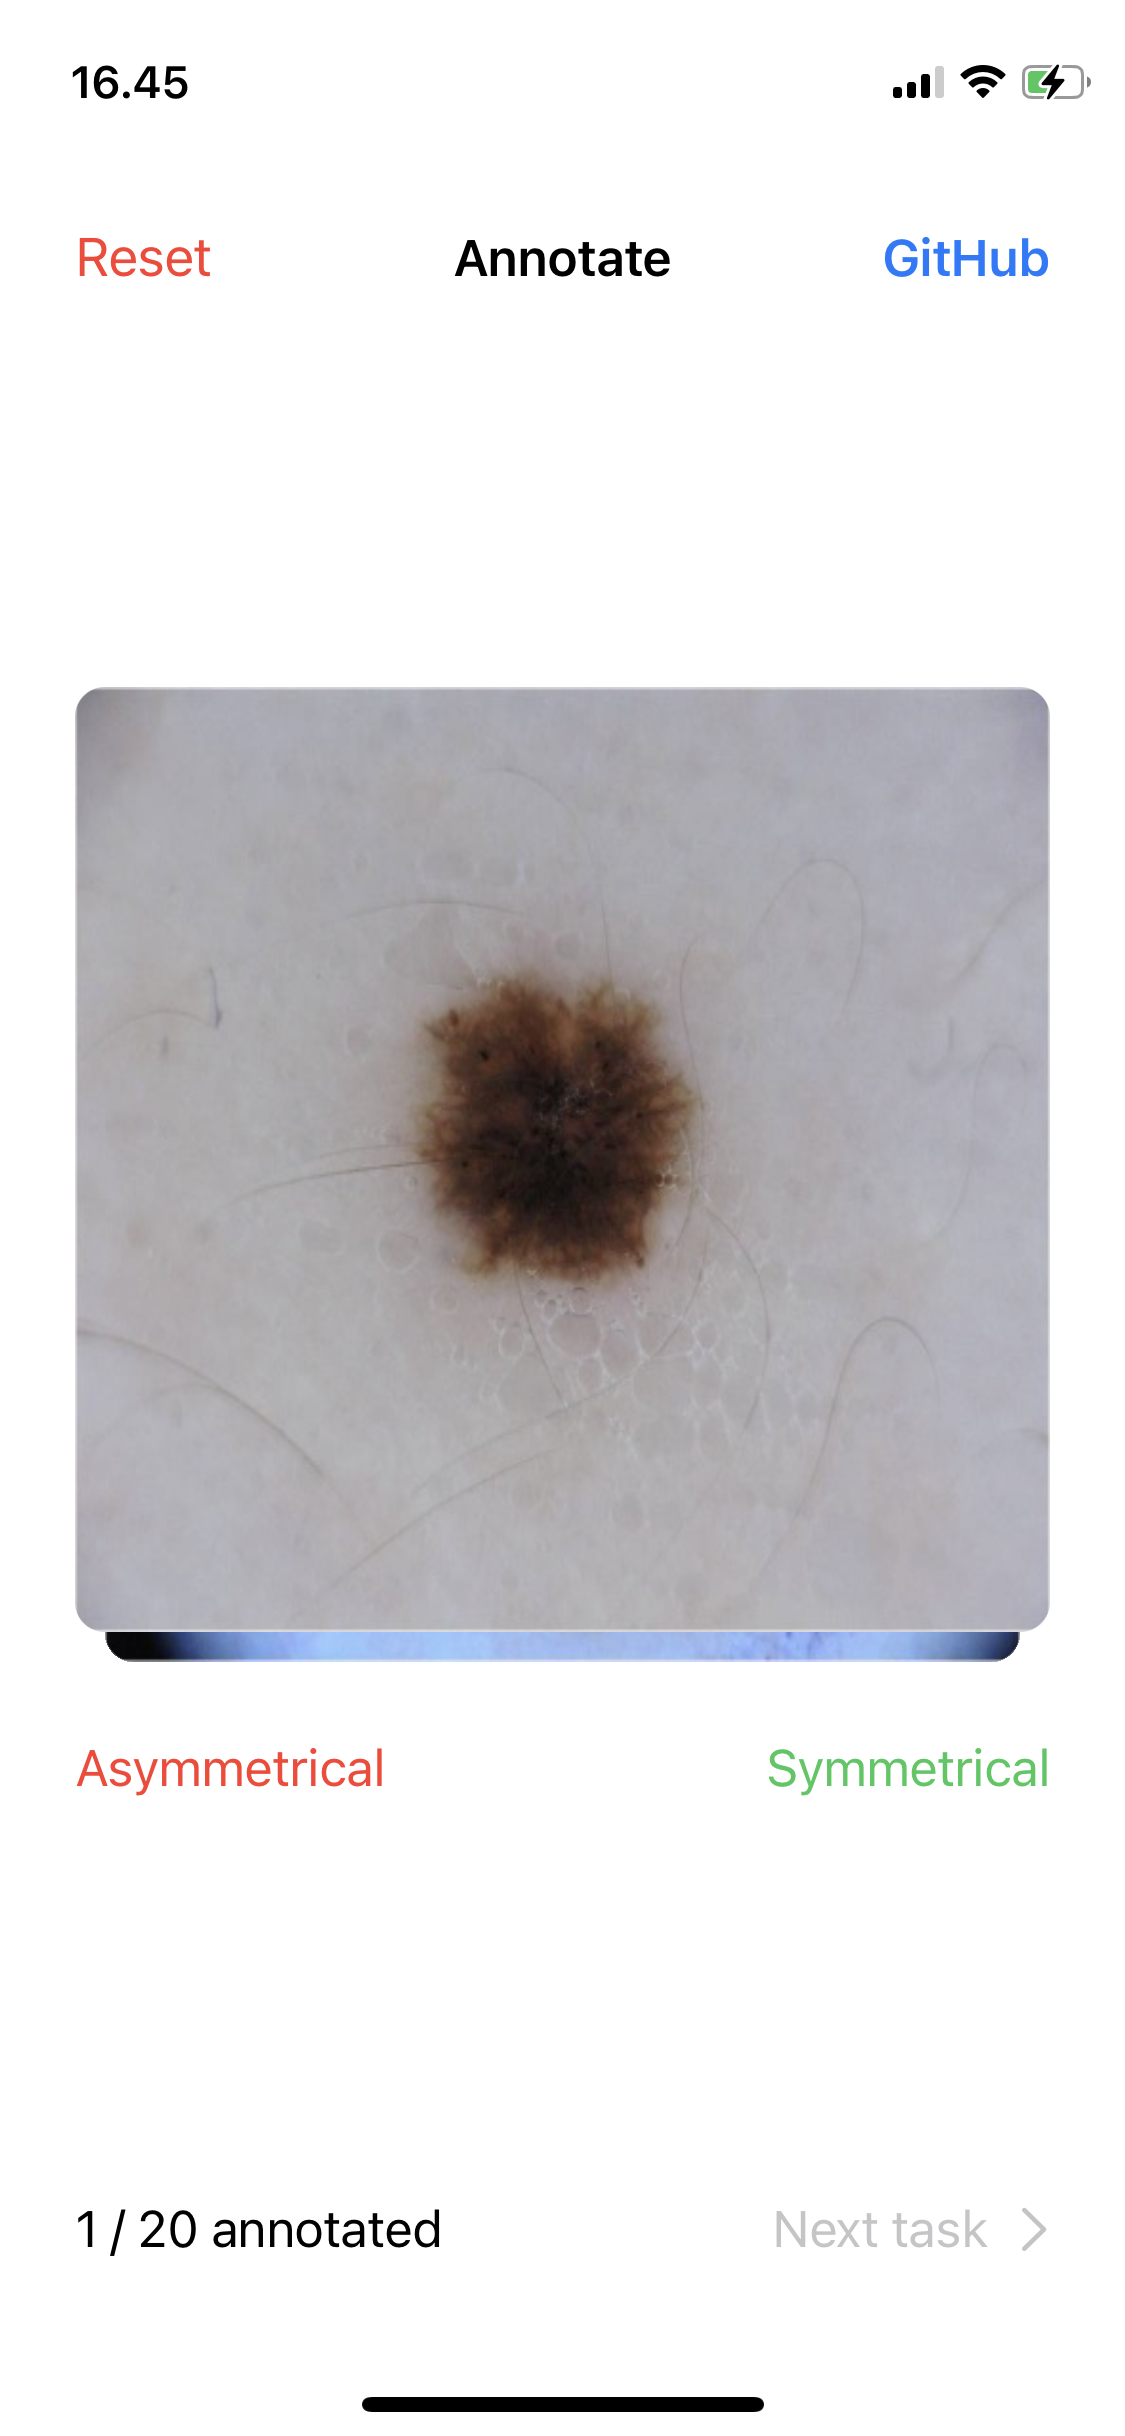
\includegraphics[width=.19\textwidth]{figures/screenshot1.png}}\hfill
\frame{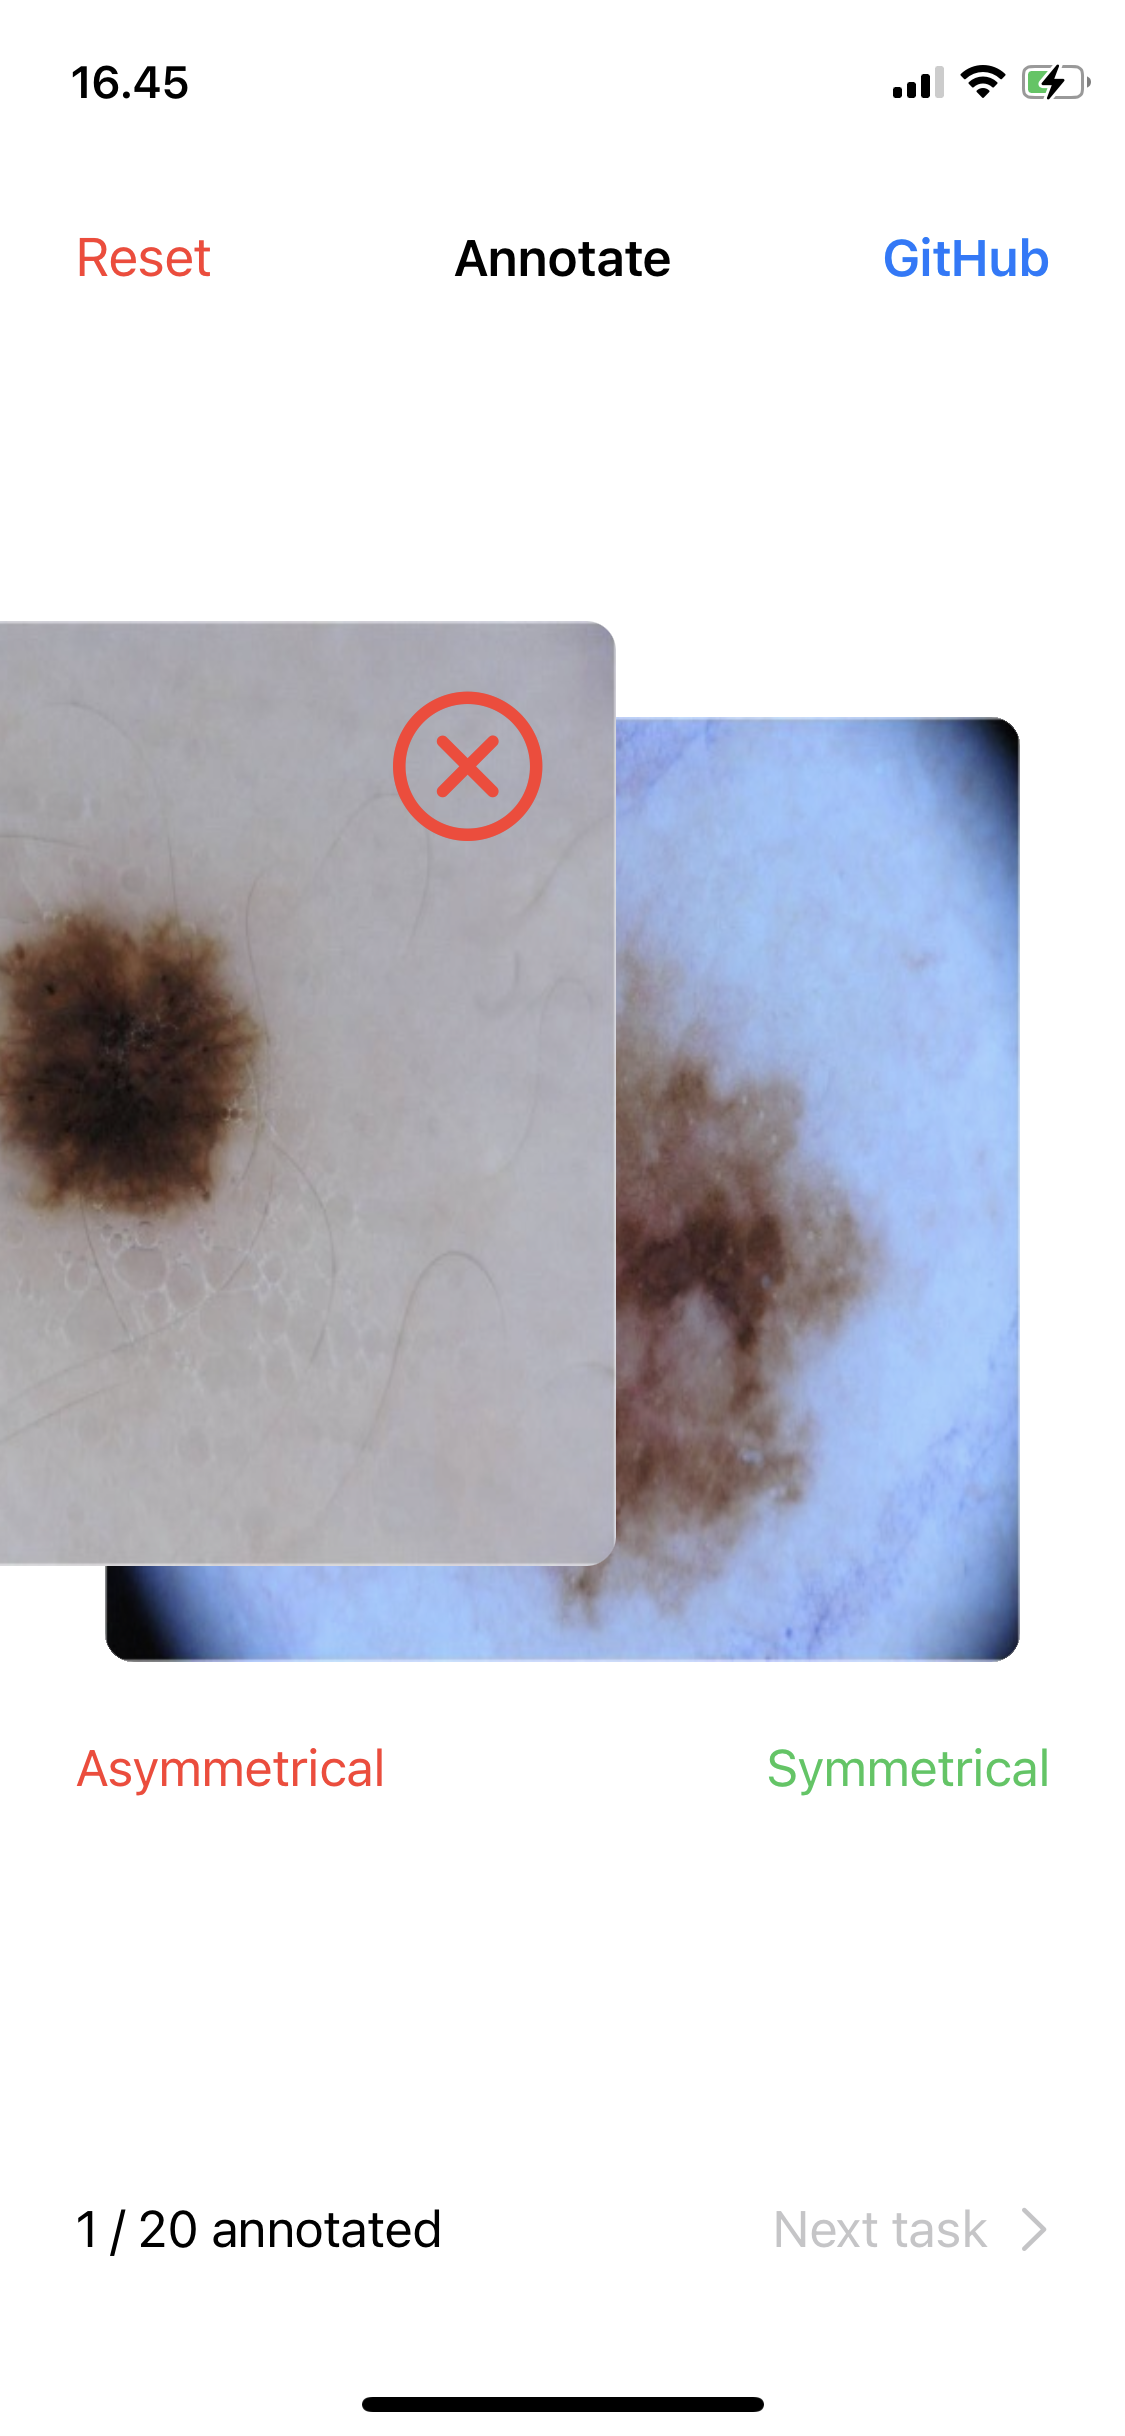
\includegraphics[width=.19\textwidth]{figures/screenshot2.png}}\hfill
\frame{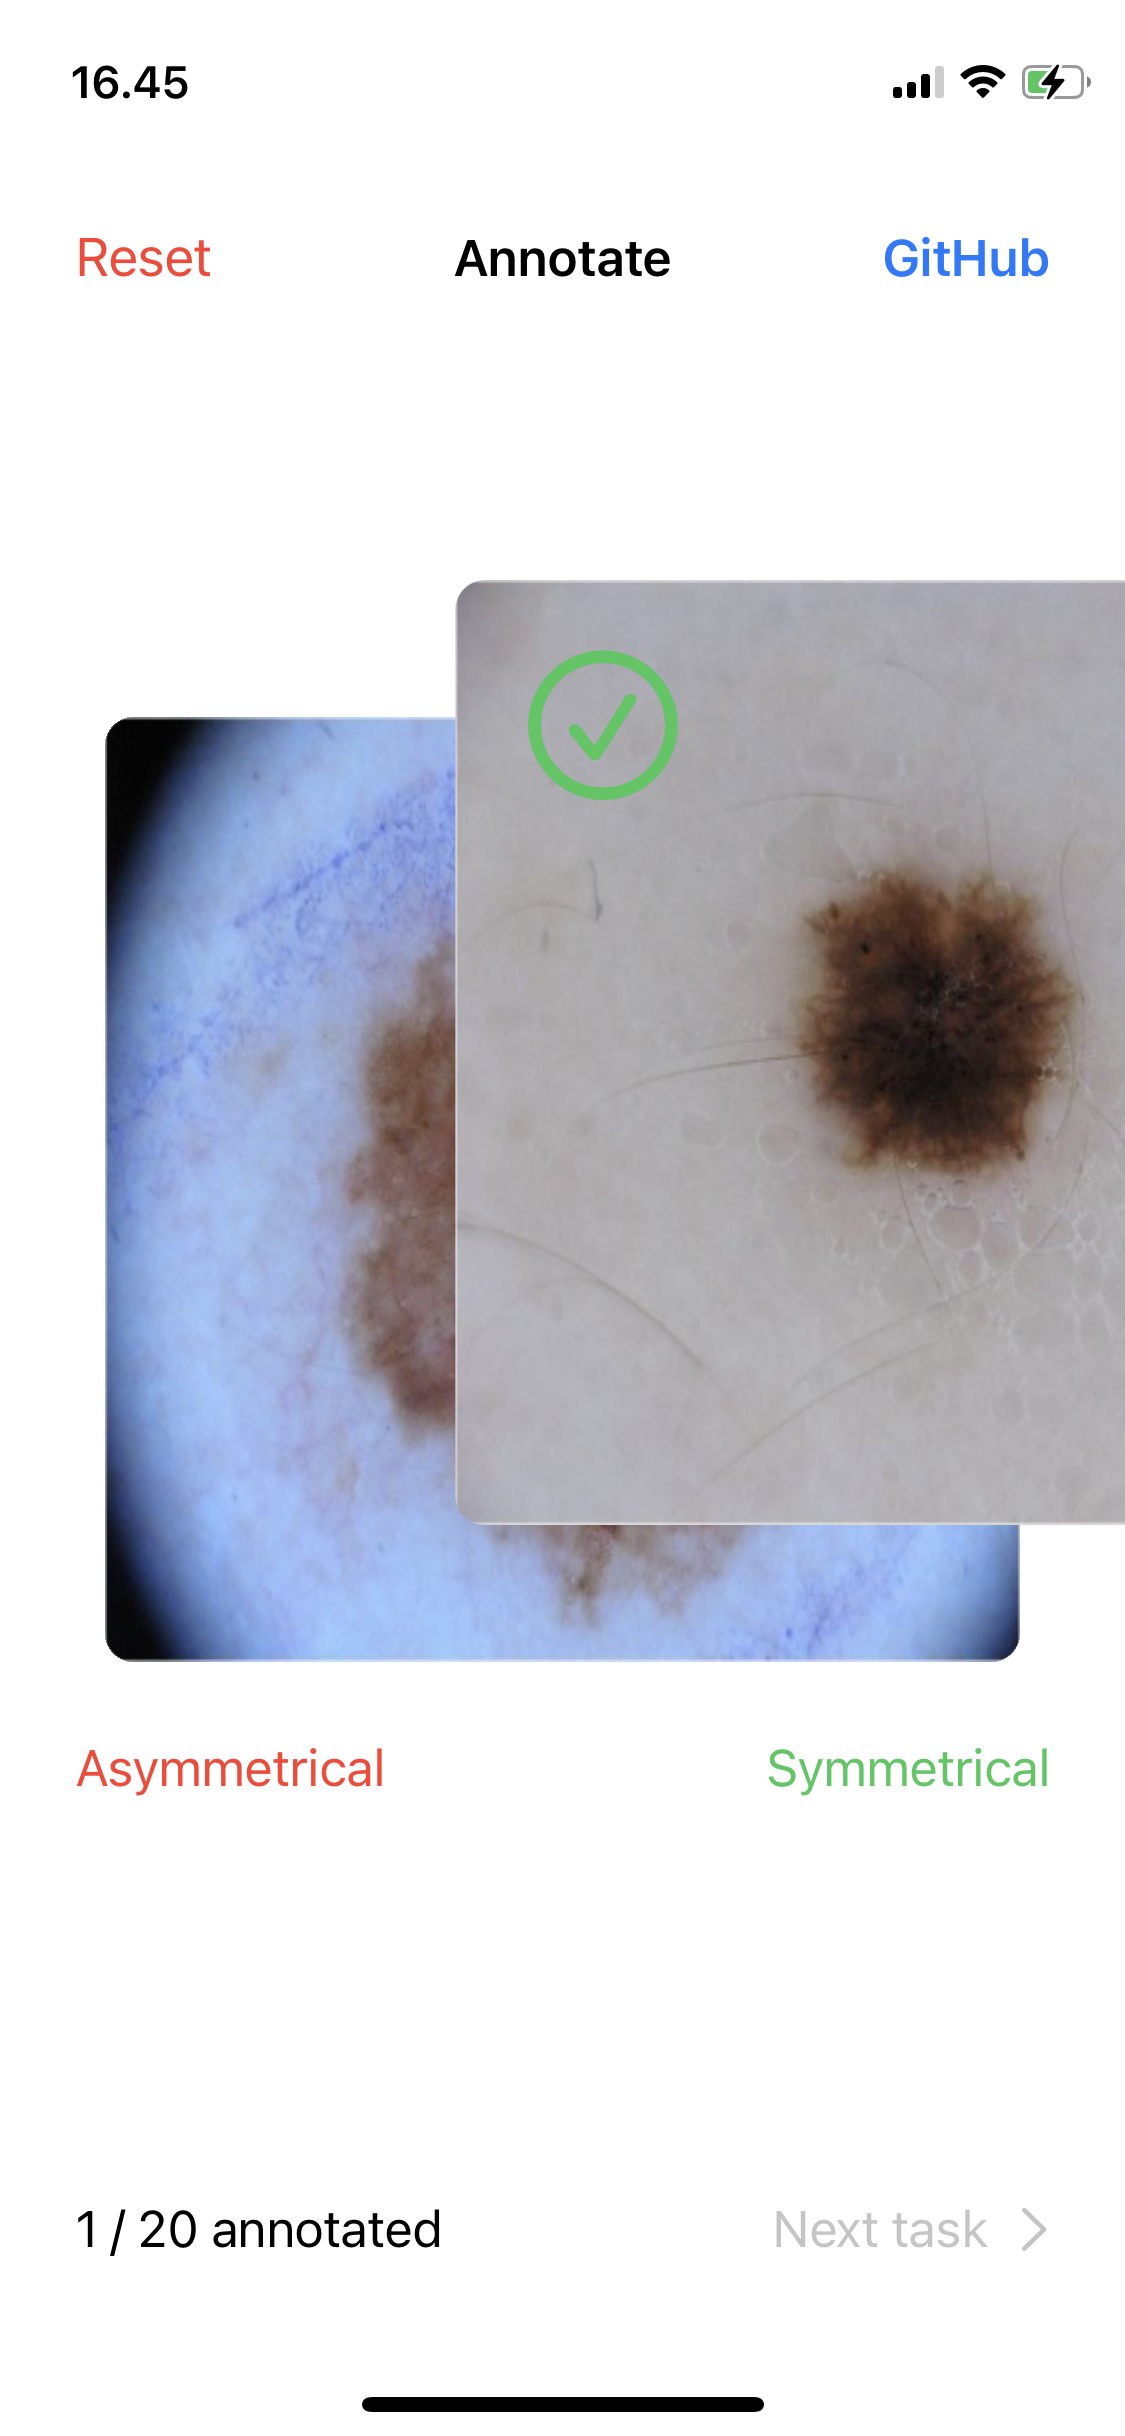
\includegraphics[width=.19\textwidth]{figures/screenshot3.png}}\hfill
\frame{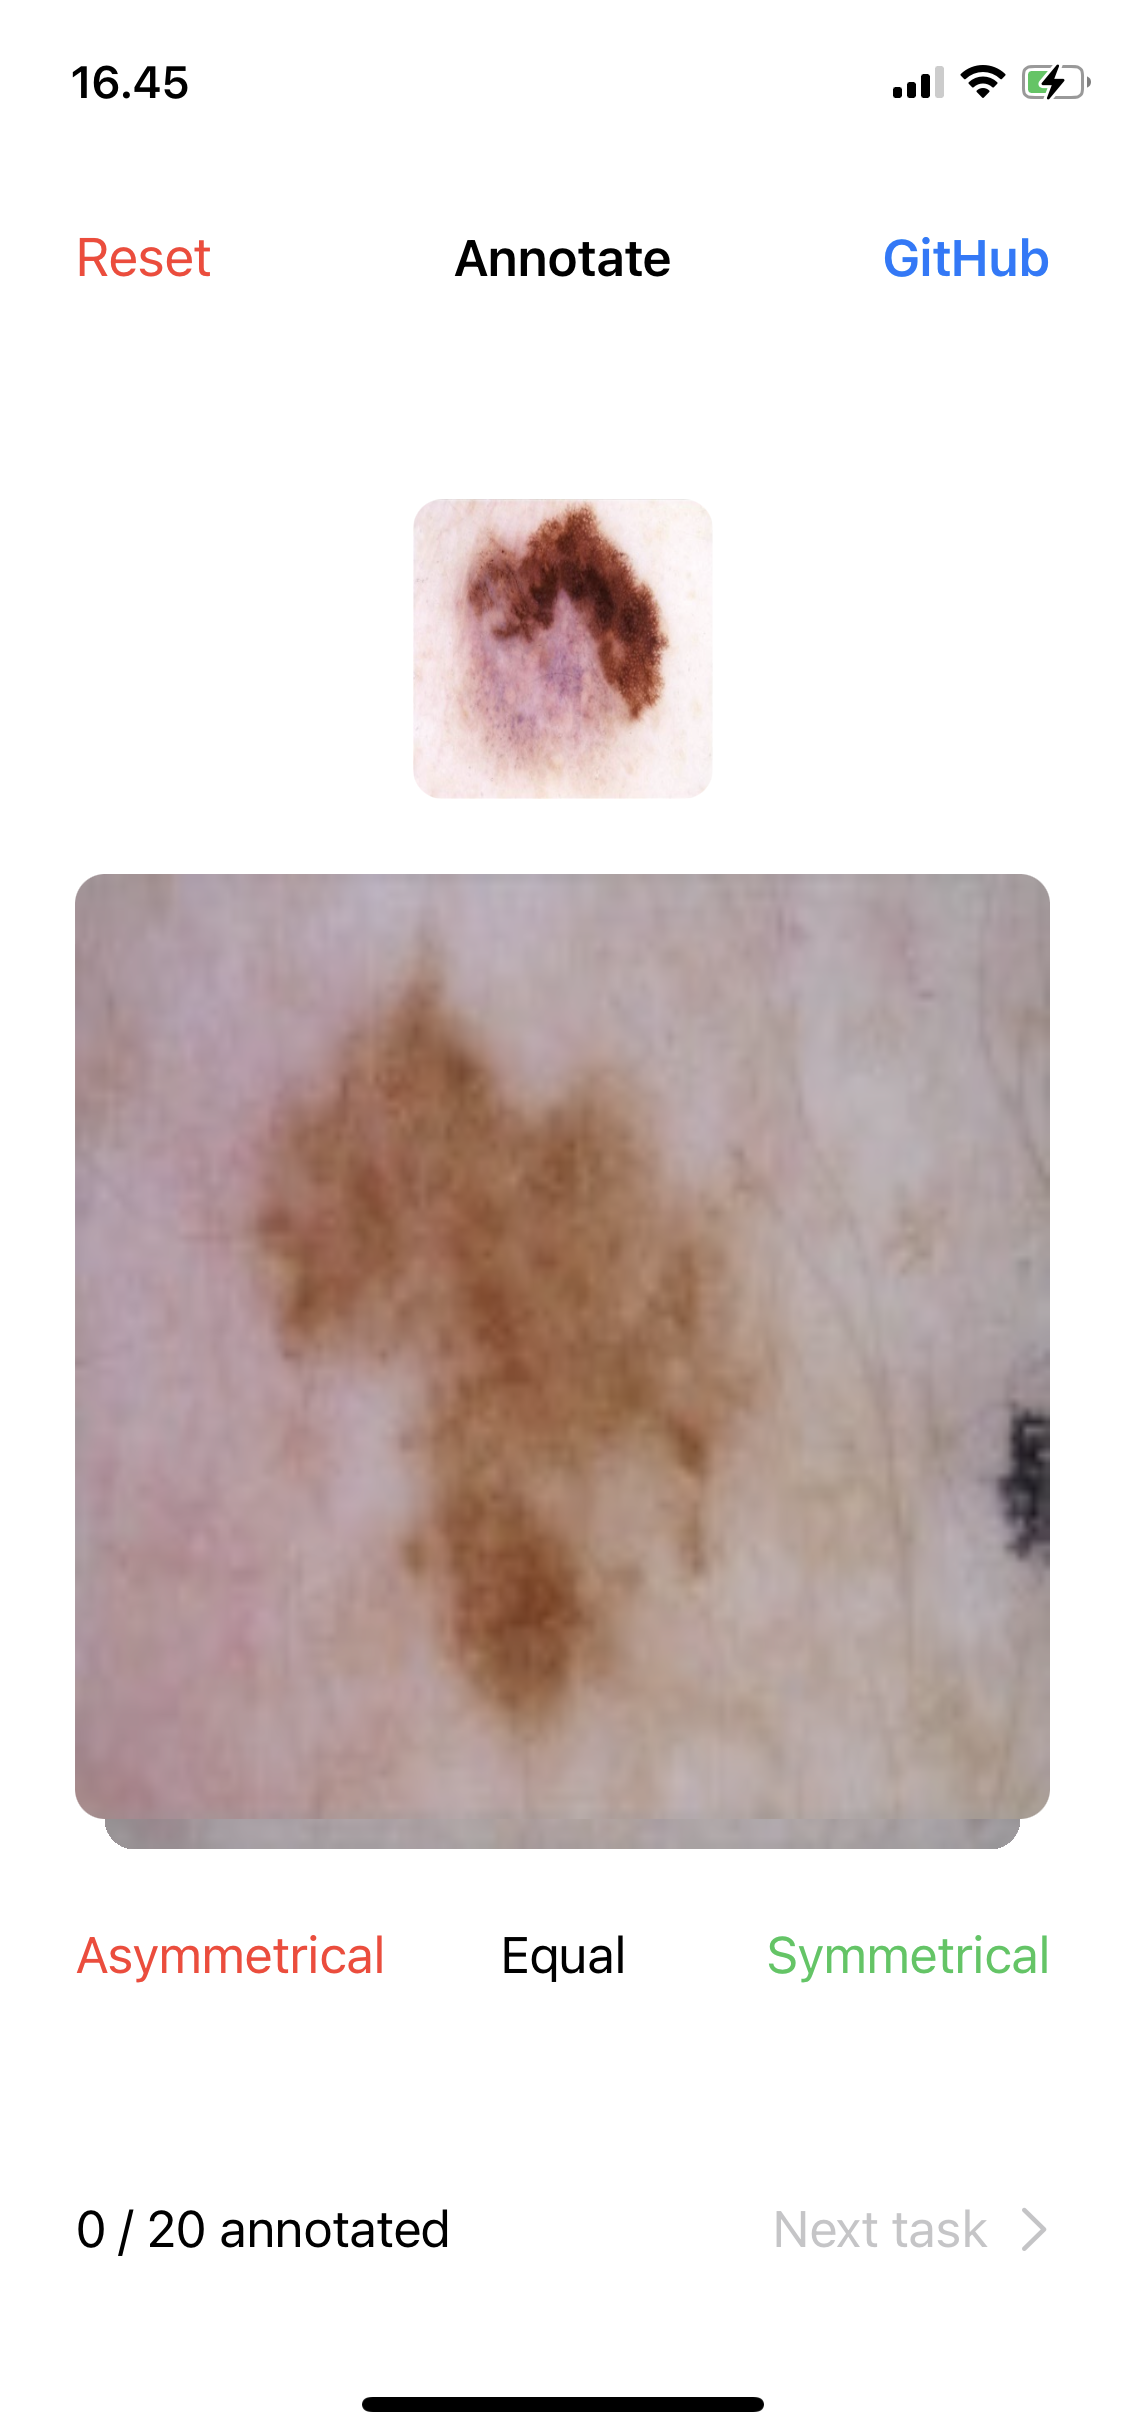
\includegraphics[width=.19\textwidth]{figures/screenshot4.png}}\hfill
\frame{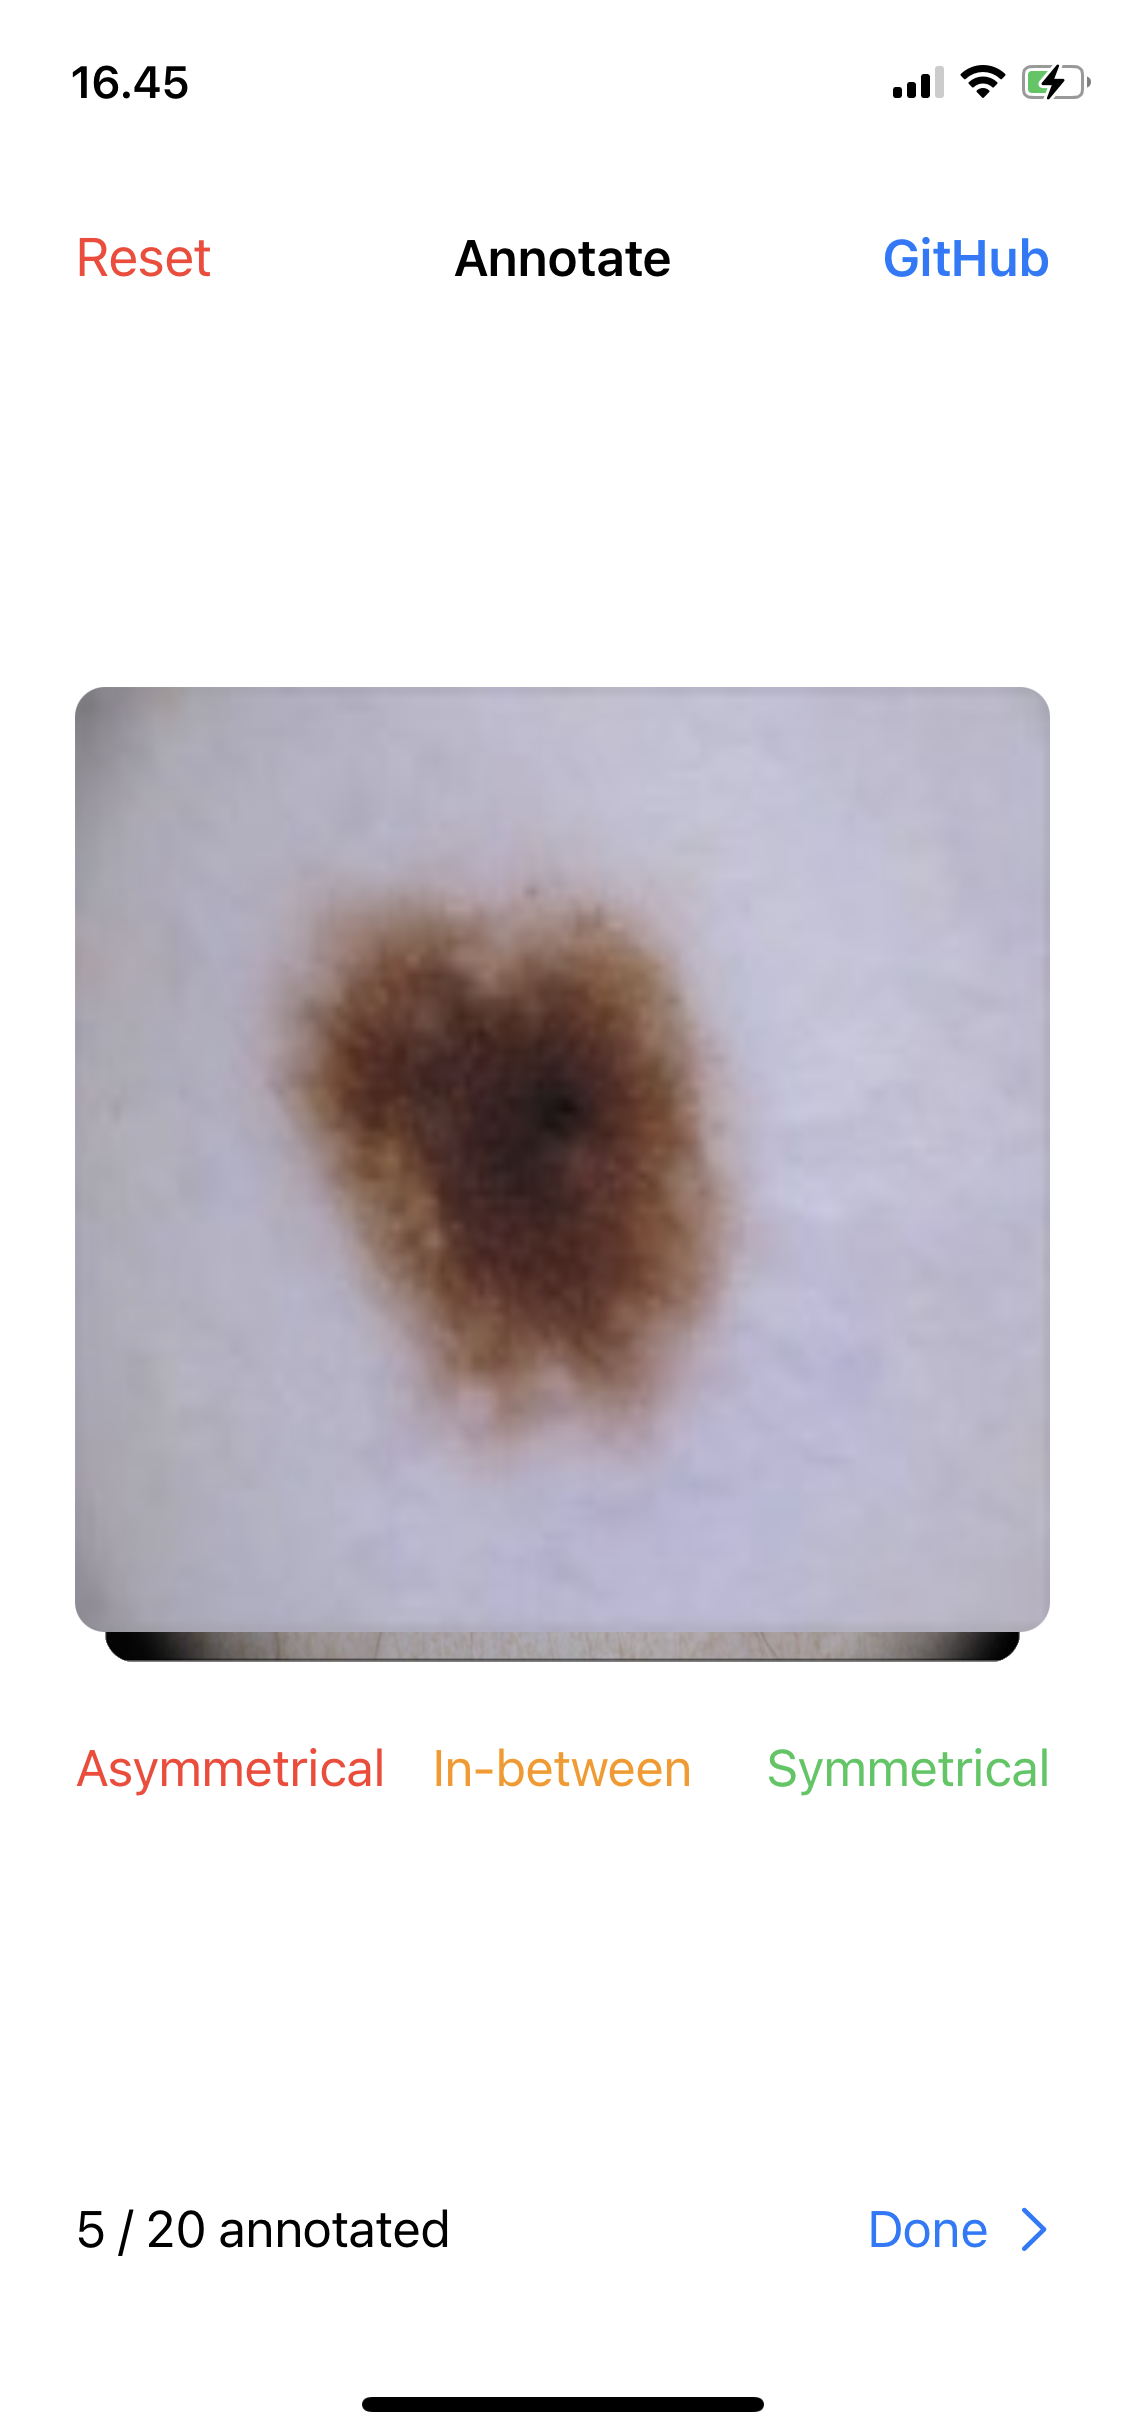
\includegraphics[width=.19\textwidth]{figures/screenshot5.png}}
\caption{Screenshots of the annotation tasks.}
\label{fig:application}
\end{figure*}

\subsection{Image Dataset}

% ISIC 2017
The ISIC 2017 Challenge \cite{ISIC2017Challenge} encouraged competitors to develop image analysis tools for melanoma classification. It consists of around 2000 melanoma images, of which a training data subset was selected to match the subset in the ENHANCE project \cite{Ralf2021ENHANCE}. This is the only dataset used in this project, as the value of each task variant is determined by how closely the annotations produced match those produced in the ENHANCE project \cite{Ralf2021ENHANCE}. \\

This subset includes 1250 images from the ISIC 2017 dataset. The ENHANCE project \cite{Hassenzahl2010Experience} produced 3 annotations per feature (asymmetry, border, color) for each of the 1250 images, resulting in 11250 annotations. Using the MTurk platform \cite{mturk}, annotation tasks were assigned to workers at random. MTurk takes a distributed approach, by assigning small tasks to a large pool of workers. This approach allows tasks to be performed concurrently, reducing the time researchers to have to wait for results, and preventing potential worker fatigue. \\

As this project aims to motivate annotators without a financial incentive, it was unrealistic to expect each annotator to classify the entire subset for each feature and each task variance. As such, a distributed approach similar to MTurk is necessary, and can be achieved by developing a system that assigns tasks to annotators based on the [in]completeness of the annotations dataset. As systems design is resource intensive and not the focus point of this project, the subset was reduced to the first 60 images, which were further split into three groups of 20 images, one group for each annotation task.

\subsection{Technical Implementation}

% systems distribution
The annotation tasks were implemented as a Swift application (see figure \ref{fig:application}). It leverages the universal and Apple platform-neutral SwiftUI framework, which allows the tasks to adapt to their platform and context of use. This application was phrased as an educational component with a subsequent three-stage annotation task component. This is the same approach as was taken Braindr \cite{Braindr}, but with the annotation divided into three tasks. \\

The tasks are designed to be distributed to a small pool of testers, reflected in the fact that a small (n=60, divided in 3) subset of images was selected. If a larger pool of crowdsourced workers were to be leveraged, a distributed systems approach would be necessary. Through this approach, annotation progress would be tracked server-side, and annotators would be assigned random subsets of images based on [in]completeness of the produced dataset.

\subsection{Study Design}

% test user sampling
Annotators were selected based on their educational background and knowledge of the subject, as I wanted to avoid testing with people who already had medical experience or an understanding of melanoma classification. They were sampled through non-saturation and non-probability convenience sampling, as defined by Sharp et al. \cite{sharp2019interaction}). Non-saturation sampling meant a limited amount of test persons were necessary, as I only needed 20 annotations per image. Non-probability sampling meant test persons were not selected based on probability, but rather selected directly by me. Convenience sampling meant test persons did not volunteer, but rather they were selected because of my accessibility to them.

\subsection{Annotation Tasks}

% Braindr.us as sample interaction
Braindr \cite{Braindr} leverages a simple and rapid bi-directional task, wherein users swipe/click left or right on each image in a procedually generated stack representing their dataset. A left swipe/click annotates the given image as "Fail", while a right swipe/click annotates the given images as "Pass". This interaction was sampled for this project, because it conforms well to different contexts of use, and can be easily varied across the scale of interaction attributes. \\

% Variances based on scale of interaction attributes
Variances of the annotation task were determined by first categorizing the Braindr \cite{Braindr} interaction relative to the attribute scale, and then finding ideating based on opposing or non-present attributes. This process lead to the development of three distinct variants: fail or pass, similarity, and Likert scale. \\

\textit{1) Fail or pass.} In this task, annotators classify an image as asymmetrical or symmetrical. It is intended to reproduce the experience of Braindr \cite{Braindr}, acting as a baseline design. Based on the interaction vocabulary, this design is fast, stepwise, instant, direct, spatially proximate, precise, and targeted. \\

\textit{2) Similarity.} In this task, annotators classify an image based on its similarity to a randomised reference image. Annotations can be asymmetrical, symmetrical, or equal to the reference image. Based on the interaction vocabulary, this design is slower and less uniform than the baseline, as a third classification is added. \\

\textit{3) Likert scale.} In this task, annotators classify an image as asymmetrical or symmetrical, with the option to classify as an intermediary between the two This approach is similar to a Likert scale. Based on the interaction vocabulary, this design is slower, less uniform and more spatially separated than the baseline, as a third classification is added and there is no unique direction or position for the annotator to target. \\

A Likert scale is a psychometric technique that measures human attitude, as defined by Joshi et al. \cite{joshi2015likert}. This scale can be either symmetric or asymmetric, meaning the classifications are either even or uneven in numbers. An asymmetric scale can contain an intermediary value, that is a value reflecting neither side of a discrete or continuous scale (see figure \ref{fig:likert}).

\pagebreak

\begin{figure}[h!]
\centering
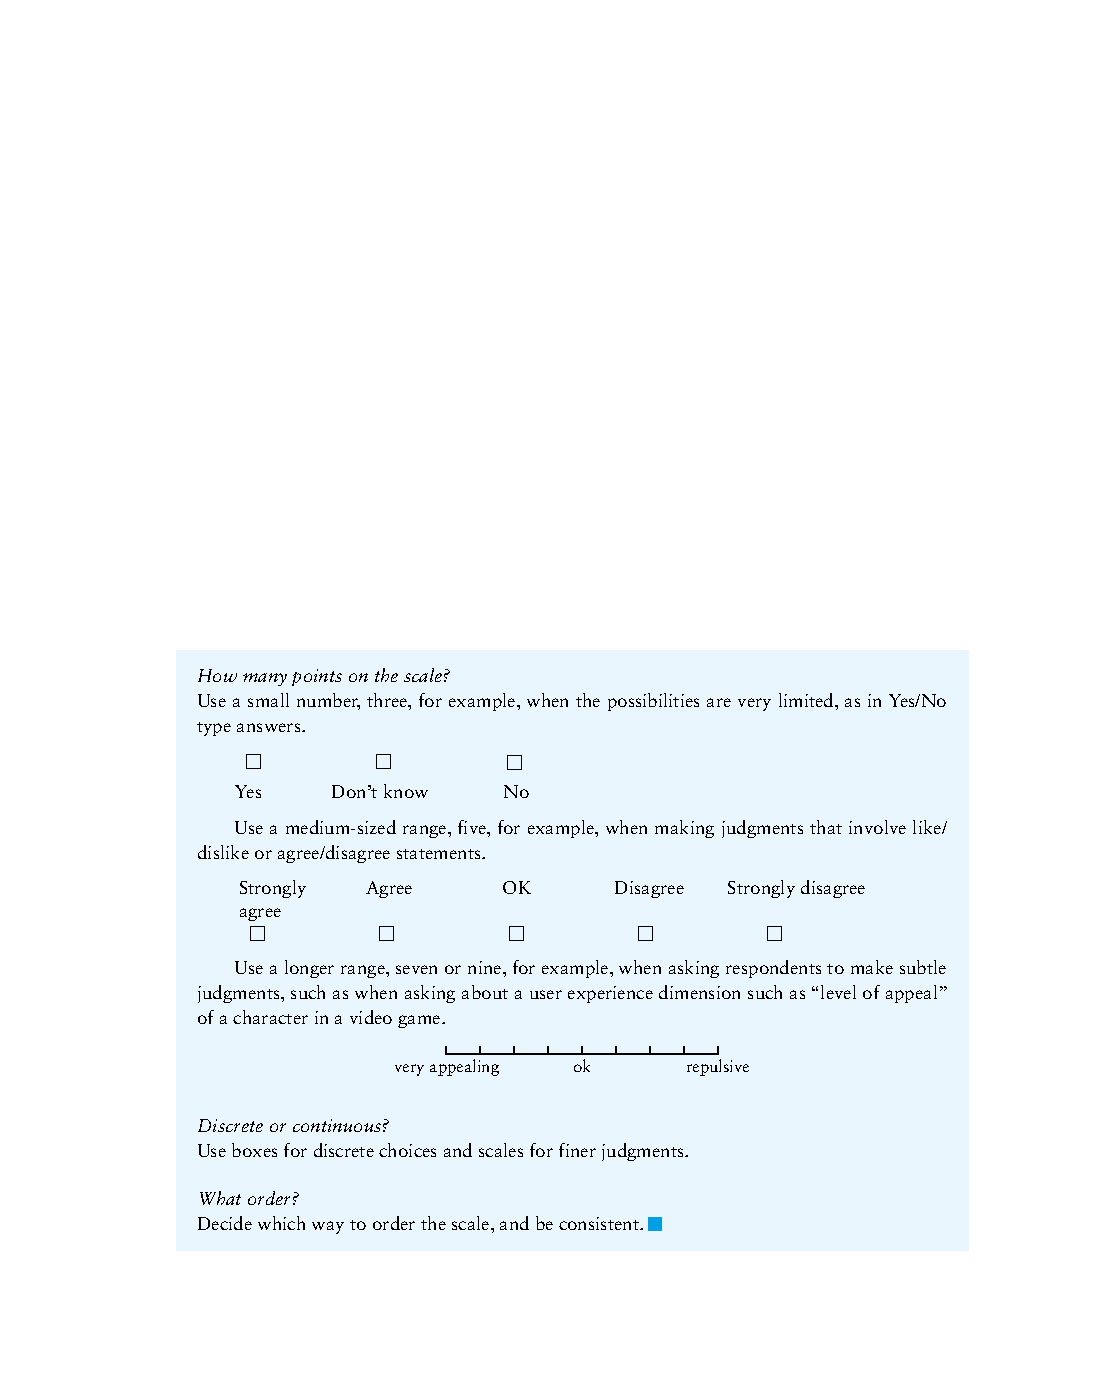
\includegraphics[width=8cm]{figures/likert.pdf}
\caption{An asymmetric Likert scale \cite{joshi2015likert}}
\label{fig:likert}
\end{figure}

The purpose of appropriating the asymmetric Likert scale for this project, was to give annotators agency and autonomy in deciding whether an annotation fit into neither of the discrete classifications. This is accomplished by providing an intermediary classification, which was notably absent from the Braindr project \cite{Braindr}.

\subsection{Evaluation}

Twenty annotators were recruited for participation in the annotation tasks, with each annotator producing a dataset for the 60 images from the ENHANCE project's \cite{Ralf2021ENHANCE} 1250 image subset of the ISIC 2017 challenge dataset \cite{ISIC2017Challenge}. In addition to producing annotations, these participants were asked to reflect on the tasks, and were encouraged to vocalise their thoughts or confusions during annotation. \\

The task variances are evaluated by comparing the resulting annotations to the results produced in the ENHANCE project \cite{Ralf2021ENHANCE}. The purpose of using a similar crowdsourcing project as reference, is to define and evaluate the data quality produced through the designed tasks. \\

This comparison consists of two datasets for each feature: \textit{asymmetry}, \textit{border}, and \textit{color}. The first reference dataset is from the ENHANCE project \cite{Ralf2021ENHANCE}, and the second dataset is produced through this experiment. Data quality is defined as indifference in annotations between the two datasets.

\end{document}